\documentclass[12pt, a4paper]{article}

\usepackage[hmargin=2.5cm, vmargin=2cm]{geometry}
\usepackage{amsthm, amssymb, mathtools, yhmath, graphicx}
\usepackage{fontspec, type1cm, titlesec, titling, fancyhdr, tabularx}
\usepackage{color}
\usepackage{unicode-math}
\usepackage{float}
\usepackage{hhline}
\usepackage{comment}
\usepackage[abbreviations]{siunitx}
\usepackage{csvsimple}
\usepackage{subcaption}
\usepackage{cleveref}
\usepackage{listings}
\definecolor{mygreen}{rgb}{0,0.6,0}
\lstset{
  basicstyle=\footnotesize\ttfamily,
  breaklines=true,
  keywordstyle=\color{blue},
  numbers=left,
  numberstyle=\tiny\color{mygray},
  commentstyle=\color{mygreen}, 
}

\usepackage[CheckSingle, CJKmath]{xeCJK}
\usepackage{CJKulem}
\usepackage{enumitem}
\usepackage{tikz}
\usepackage[siunitx]{circuitikz}
\usepackage{wrapfig}
\usepackage{sourcecodepro}
%\setCJKmainfont[BoldFont=cwTex Q Hei]{cwTex Q Ming}
%\setCJKsansfont[BoldFont=cwTex Q Hei]{cwTex Q Ming}
%\setCJKmonofont[BoldFont=cwTex Q Hei]{cwTex Q Ming}
\setCJKmainfont[BoldFont=cwTeX Q Hei]{cwTeX Q Ming}
\setmonofont{Source Code Pro}

\def\normalsize{\fontsize{12}{18}\selectfont}
\def\large{\fontsize{14}{21}\selectfont}
\def\Large{\fontsize{16}{24}\selectfont}
\def\LARGE{\fontsize{18}{27}\selectfont}
\def\huge{\fontsize{20}{30}\selectfont}

\newtheorem{lemma}{Lemma}

%\titleformat{\section}{\bf\Large}{\arabic{section}}{24pt}{}
%\titleformat{\subsection}{\large}{\arabic{subsection}.}{12pt}{}
%\titlespacing*{\subsection}{0pt}{0pt}{1.5ex}

\parindent=24pt

\DeclarePairedDelimiter{\abs}{\lvert}{\rvert}
\DeclarePairedDelimiter{\norm}{\lVert}{\rVert}
\DeclarePairedDelimiter{\inpd}{\langle}{\rangle}
\DeclarePairedDelimiter{\ceil}{\lceil}{\rceil}
\DeclarePairedDelimiter{\floor}{\lfloor}{\rfloor}

\newcommand{\unit}[1]{\:(\text{#1})}
\newcommand{\df}[1]{\mathop{}\!\mathrm{d^#1}}
\newcommand{\img}{\mathrm{i}}
\newcommand{\dD}{\mathrm{d}}
\newcommand{\dI}{\,\mathrm{d}}

\title{ \bf {\Huge Signal and System}\\ MATLAB Homework \#2}
\author{B02901178 江誠敏}

\begin{document}

\maketitle

\section{Problem 1}
\begin{enumerate}[label=(\alph*)]
  \item {\bf Plot $x[n]$.} \\[12pt]

    \begin{figure}[H]
      \centering
      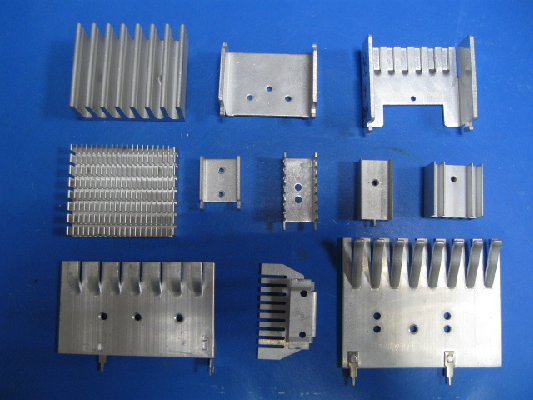
\includegraphics[width=0.6\textwidth]{p1.jpg}
      \caption{Plot of $x[n]$.}
    \end{figure}
  \item {\bf Plot the magnitude response of the DFT of $x$ during $[−N_1, N_1]$. The zero
    frequency should be centered in your plot. Observe the Gibbs phenomenon here.} \\[12pt]
    \begin{center}
    \begin{figure}[H]
      \centering
      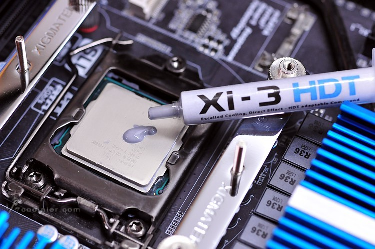
\includegraphics[width=0.6\textwidth]{p2.jpg}
      \caption{Plot of the magnitude response.}
    \end{figure}
    \end{center}

  \item {\bf We define the overlapping factor $K$ so that $n \in \{−KN_1, −KN_1+1,\cdots , 0, \cdots , KN_1−1, KN_1\}$.
    Please repeat part (a) and (b) with $K = 16$ and fixed $T_s$, then compare the
  Gibbs phenomenon in (b).}\\[12pt]
    \begin{center}
    \begin{figure}[H]
      \begin{subfigure}{0.48\textwidth}
        \centering
        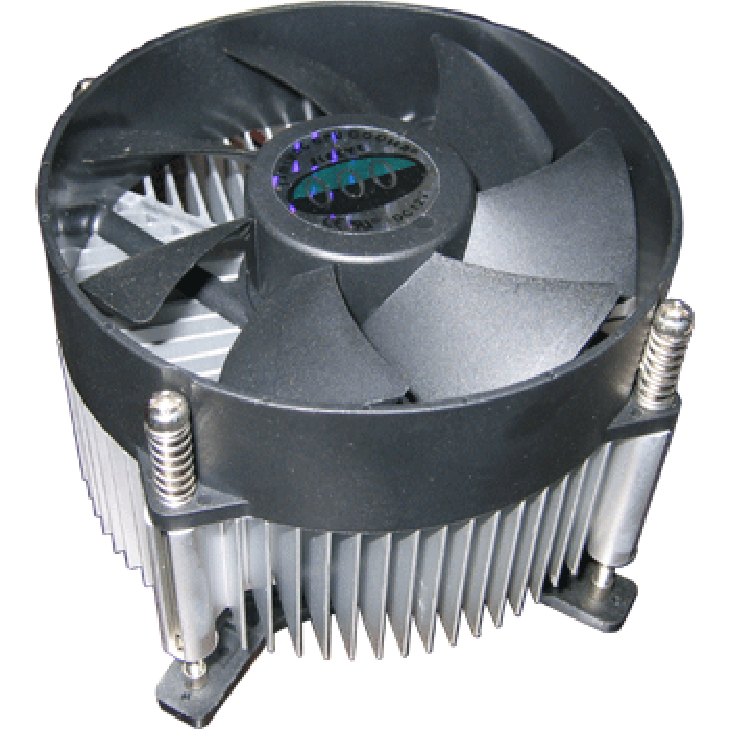
\includegraphics[width=\textwidth]{p3.jpg}
        \caption{Plot of $x[n]$.}
      \end{subfigure}%
      \begin{subfigure}{0.48\textwidth}
        \centering
        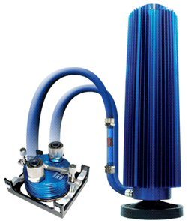
\includegraphics[width=\textwidth]{p4.jpg}
        \caption{Plot of the magnitude response.}
      \end{subfigure}
    \end{figure}
    \end{center}

    The distortion width is smaller, but the maximum height (i.e the maximum error) remain the same.

\section{Problem 2}
\begin{enumerate}[label=(\alph*)]
  \item {\bf Plot $x[n]$ when $ n \in \mathcal{N} $.}    \\[12pt]
    \begin{center}
    \begin{figure}[H]
      \centering
      \includegraphics[width=0.6\textwidth]{p5.jpg}
      \caption{Plot of $x[n]$.}
    \end{figure}
  \end{center}

\item {\bf Now let $b = 0.2$ and $N = 3$. Assuming that at $n = 0$ and we initialize the
  EWMA filter with $x[−1] = \cdots = x[−N] = 0$, plot the output of the filter for $n \in \mathcal{N}$.}
    \\[12pt]
    \begin{center}
    \begin{figure}[H]
      \centering
      \includegraphics[width=0.8\textwidth]{p6.jpg}
      \caption{Plot of the output after filter.}
    \end{figure}
  \end{center}

\item {\bf Repeat part (b) with $b = 0.2$ and $N = 10$.}    \\[12pt]
    \begin{center}
    \begin{figure}[H]
      \centering
      \includegraphics[width=0.8\textwidth]{p8.jpg}
      \caption{Plot of the output after filter.}
    \end{figure}
  \end{center}
  
\item {\bf Comment on the relationship between the filter outputs in parts (b) and (c)
  with the original signal $s[n]$.} \\[12pt]
  After the filter, the signal looks slightly smoother, but is still similar to the
  origin input, since the decay rate $b$ is small (so it decay fast!).

  Also because the decay rate $b$ is too small, $N = 3$ and $N = 10$ gives almost the
  same result.

\clearpage
\item {\bf Please repeat parts (b), and (d) with $b = 0.5$ and $N = 3$.} \\[12pt]
  \begin{center}
    \begin{figure}[H]
      \centering
      \includegraphics[width=0.8\textwidth]{p10.jpg}
      \caption{Plot of the output after filter.}
    \end{figure}
  \end{center}
  The output is much smoother and closer to the signal without the noise compare to the input.

\item {\bf What is the effect of increasing $b$? What about increasing $N$?} \\ [12pt]
  Increasing $b$ tends to make the output smoother. \\
  Increasing $N$ at small $N$ could also let the output become smoother,
  provided that $b$ is not too small.
\end{enumerate}
\end{document}

